\documentclass[12pt,fleqn]{article}
\usepackage{xiiiemc}
\usepackage{natbib}
\usepackage{fancyhdr}
\usepackage{color}
\usepackage{wallpaper}
\usepackage{titlesec}   %% Define space between paragraph e section
\usepackage{float} 	%% Use to fix Figure or Table: ex: \begin{table}[H]
%%%%Don't edit this block. It reduces the spacing between the lines of the references
\let\OLDthebibliography\thebibliography
\renewcommand\thebibliography[1]{\OLDthebibliography{#1} \setlength{\parskip}{0pt}\setlength{\itemsep}{0pt plus 0.3ex}}

%%-----------------------------------------------EDIT-----------------------------------------------
\title{COMPARISON OF THE DIFFERENTIAL EVOLUTION AND SIMULATED ANNEALING ALGORITHMS APPLIED TO THE CONSTRUCTAL DESIGN OF DOUBLE-T SHAPED CAVITIES}

%%-----------------------------------------------EDIT----------------------------------------------
\author
    {\rm \begin{tabular}{l}
    \textbf{Gill Velleda Gonzales}$^{1,2}$ - {\textnormal gillgonzales@ifsul.edu.br}\\%
    \textbf{Elizaldo Domingues dos Santos}$^{2}$ - {\textnormal elizaldodossantos@gmail.com}\\
    \textbf{Antônio J. Silva Neto}$^{3}$ - {\textnormal ajsneto@iprj.uerj.br}\\
    {\fontsize{11}{0}\selectfont $^{1}$Instituto Federal Sul-Rio-Grandense - Campus Santana do Livramento, RS, Brazil}\vspace*{-0.05cm} \\
    {\fontsize{11}{0}\selectfont $^{2}$Universidade Federal do Rio Grande - PPG em Modelagem Computacional, Rio Grande, RS, Brazil}\vspace*{-0.05cm}\\
    {\fontsize{11}{0}\selectfont $^{3}$Universidade do Estado do Rio de Janeiro, Instituto Politécnico - Nova Friburgo, RJ, Brazil}
  \end{tabular}}
%%----------------------------------------------------------------------------------------------

\fancypagestyle{firspagetstyle}
{
	\lhead{}
	\fancyhead[C]{%
		
\includegraphics[width=0.75\linewidth]{logo}\\%
		{\scriptsize \fontfamily{phv}\fontseries{b}\selectfont \color[rgb]{0.45,0.45,0.45}
		08 a 11 de Outubro de 2018\\
		Instituto Federal Fluminense\\
		Búzios - RJ\\
	    }
	}
	\renewcommand{\headrulewidth}{0.0pt}
	\fancyfoot[C]{\footnotesize \parbox{15cm} {\centering  \fontsize{7.5}{0}\selectfont \it Anais do XXI ENMC – Encontro Nacional de Modelagem Computacional e IX ECTM – Encontro de Ciências e Tecnologia de Materiais,  Búzios, RJ – 08 a 11 Outubro 2018}} % \ttfamil
	\rhead{}
}


\begin{document}
\maketitle

\thispagestyle{firspagetstyle}

\fancyhead[L]{\footnotesize{\fontsize{7.5}{0}\selectfont \it XXI ENMC e IX ECTM\\
	08 a 11 de Outubro de 2018\\
	Instituto Federal Fluminense – Búzios - RJ\\}}
\renewcommand{\headrulewidth}{0.0pt}
\fancyfoot[C]{\footnotesize \parbox{15cm} {\centering  \fontsize{7.5}{0}\selectfont \it Anais do XXI ENMC – Encontro Nacional de Modelagem Computacional e IX ECTM – Encontro de Ciências e Tecnologia de Materiais,  Búzios, RJ – 08 a 11 Outubro 2018}} % \ttfamil
\rhead{}

\begin{abstract}
In this paper, it is analyzed the application of two meta-heuristic methods, Differential Evolution and Simulated Annealing, for the geometric optimization in a heat transfer problem. The optimization problem is defined by the Constructal Design method, that determines the objective and constraints in the optimization process, as well as, the degrees of freedom of the geometry that is optimized. The main purpose of this work is the comparison between the results of this two meta-heuristics, mainly the reproduction of the degrees of freedom effect over the optimal geometry, and the thermal performance of the computational domain. The experiment consists in performing thirty runs of each algorithm, with different values for the configuration parameters, and also four versions of Differential Evolution and five versions of Simulated Annealing. The optimization results show that the meta-heuristic algorithm and its parameter configuration can lead to the wrong interpretation of the effect of degrees of freedom over optimal geometry. It is possible to conclude that the algorithm of Differential Evolution with a specific parameter configuration achieved the best and most robust results than the others algorithm. Therefore, the significant contribution here is the recommendation of the more reliable meta-heuristic, and its correct parameters for the heat transfer problem considered.
\end{abstract}

\keywords{\em{Heat Transfer, Constructal Design, Simulated Annealing, Differential Evolution, Geometric Optimization }}

\pagestyle{fancy}

\section{INTRODUCTION}
The geometric optimization of cooling cavities inside a solid with heat generation was first proposed by \cite{Biserni2004}. Through by the Constructal Design (CD) method, the elementary geometry of C-shaped and T-shaped cavities was evaluated. The CD method is based on the Constructal Theory. According to its author, \citep{Bejan}, there is a physical principle that defines the geometries in flow systems, and this principle determines the shapes and structures that emerge in nature. The Constructal Law explains that for a finite-size flow system to persist in time (to survive) its configuration must evolve in such a way that it provides easier access to the currents that flow through it \citep{Bejan}. The CD method is not an optimization method and determines the degrees of freedom which varies in the geometric optimization process and depends on the constraints to which this optimization is submitted to. The optimization is performed by an optimization method, e.g., Exhaustive Search (ES).

Employing the CD method to determine the objectives and constraints of the optimization process, more complex cavities have been evaluated \citep{Biserni2007}. Comparing the results between different shapes of cavities, kept the same constraints, it is noted that a more complex cavity geometry leads to the gain in the thermal performance, as can be seen in the complex and multi-cavity studies \citep{Lorenzini2012,Xie2010}. However, complex cavities need more degrees of freedom and require more computational effort in the optimization process. Therefore, for complex cavities, meta-heuristic methods are used as alternative methods to ES. \cite{Lorenzini2014} use Genetic Algorithm (GA) to evaluate the more complex problem in the Y-shaped cavity optimization including a convective parameter. The GA also was performed with CD to the optimization and analyses of morphing fins coupled with a heat generating body in \cite{Biserni2017}. \cite{Gonzales2015} analyses the performance of different parameters of Simulated Annealing (SA) algorithm in the geometric optimization of a Y-shaped cavity. The work of \cite{Gonzales2015} compares various parameters of the Cooling Schedule (CS) and proposes a hybrid parameter that showed best results than GA for a Y-shaped cavity. In the paper of \cite{Gonzales2017}, was performed a comparison between the Luus-Jaakola and SA algorithms with hybrid parameters of CS applied in the Double-T shaped cavity optimization. The results showed the best performance of the SA algorithm configured with the hybrid parameter of Cooling Schedule.

In the present work, the meta-heuristic of SA is compared with the Differential Evolution (DE) algorithm, applied jointly with CD, to the geometric optimization of the Double-T shaped cavity. The Double-T Shaped cavity was first proposed by \cite{Gonzales2015b}, and the SA was used in the geometric optimization. The two algorithms are performed with distinct parameters, and then the comparison is made between the variations of SA and DE. The best versions for each meta-heuristic are then compared. The SA variations differ in the Cooling Schedule (CS) parameter, and five distinct CS are performed. Different versions of the DE algorithm are compared too. The DE variations differ in the crossover and mutation operators, and four DE algorithms are performed. The double-T shaped cavity has five degrees of freedom (DOFs) that define the cavity geometry ($H/L$, $H_{0}/L_{0}$, $H_{1}/L_{1}$, $H_{2}/L_{2}$ and $S_{1}/H_{0}$). Four and five DOFs are optimized, and each algorithm achieves the curve of the effect of DOF over optimal geometry and thermal performance. The results for each algorithm are registered in a database and analyzed. Therefore, the comparison between the results of the algorithms is performed through the effect of DOF over optimal geometry, not just the minimum temperature.  Then, the better algorithm is the one that reproduces this effect with more reliable results.

\section{MATHEMATICAL AND NUMERICAL MODEL}


Figure \ref{figure01} shows the heat transfer problem of interest, that consists in a conducting body in the two-dimensional configuration, with the third dimension, with length $W$, perpendicular to the plane of the figure. The solid domain has a constant and uniform internal heat generation with the volumetric rate given by $q^{'''}(Wm^{\tiny -3})$. The solid has a constant thermal conductivity k. The outer surfaces of the solid are perfectly insulated, corresponding to adiabatic conditions. In this case, the heat can only be removed through the double-T shaped cavity, which is kept at a minimum temperature $(\theta_{min})$. The minimal temperature of the cavity may be kept with the flow of refrigerant fluid through the cavity, changing phase at a low temperature. For the sake of simplicity, the heat transfer coefficient on the cavity wall is assumed to be sufficiently large so that the convective resistance can be neglected in comparison to the solid conduction resistance.

\begin{figure}[H]
\centering
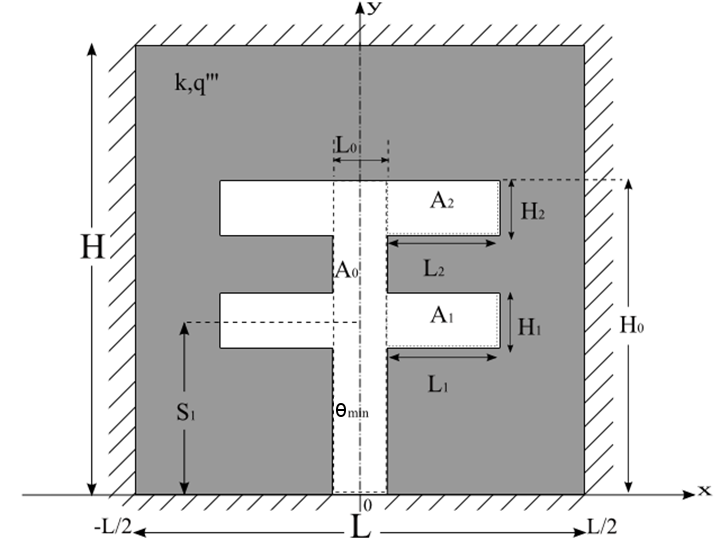
\includegraphics[width=0.6\linewidth]{imgs/duplo_t.png}
\caption{ {\small Computational domain of Double-T shaped cavity.}}
\label{figure01}
\end{figure}

The objective of the analysis is to determine the optimal geometry ($H/L$, $H_{0}/L_{0}$, $H_{1}/L_{1}$, $H_{2}/L_{2}$ and $S_{1}/H_{0}$) that is characterized by the minimum global thermal resistance $(\theta_{max} - \theta_{min})/(q^{'''}A)$. According to the CD this optimization can be subjected to the constraints of the total area and cavity area, represented respectively by:

\begin{equation}
A = HL \label{area_total}
\end{equation}
\begin{equation}
A_{c} = A_{0} + 2A_{1} + 2A_{2} \label{area_cavidade}
\end{equation}
The fraction of the cavity area with respect to the total area is given by:
\begin{equation}
\phi_{c} = A_{c}/A \label{fi}
\end{equation}
For the determination of the temperature field in the solid domain, it is necessary to solve the heat conduction equation given by:
\begin{equation}
\frac{\partial^{2} \theta}{\partial \tilde{x}^{2}}+\frac{\partial^{2} \theta}{\partial \tilde{y}^{2}}+1=0\label{calor}
\end{equation}

For the sake of brevity, the equations with dimensionless variables, the equations of boundary conditions of null flux in the solid outer surfaces, as well as, the equations of boundary conditions of minimal temperature in the cavity wall can be seen in the study by \cite{Gonzales2015b}, and are not reproduced here. The aim is to minimize the maximal excess temperature represented by the following equation:

\begin{equation}
\tilde{\theta}_{max}=\frac{\theta_{max}-\theta_{min}}{q^{'''}\cdot\frac{A}{k}}\label{fo}
\end{equation}

The determination of $\tilde{\theta}_{max}$ is needed to optimize the five degrees of freedom ($H/L$, $H_{0}/L_{0}$, $H_{1}/L_{1}$, $H_{2}/L_{2}$ and $S_{1}/H_{0}$) submitted to the corresponding constraints of the cavity area ($\phi_{c}$, $\phi_{1}$ and $\phi_{2}$) and the total solid area. In this paper are optimized the five DOFs ($H/L$, $H_{0}/L_{0}$, $H_{1}/L_{1}$, $H_{2}/L_{2}$ and $S_{1}/H_{0}$). The function represented by Eq. (\ref{fo}) is determined numerically by solving Eq. (\ref{calor}) for the temperature field in every assumed configuration ($H/L$, $H_{0}/L_{0}$, $H_{1}/L_{1}$, $H_{2}/L_{2}$ and $S_{1}/H_{0}$), and calculating $\tilde{\theta}_{max}$ to see whether its value may be minimized by varying the configuration. The numerical solution is performed with the Finite Element Method (FEM)\citep{Reddy1994}, based on linear triangular elements, available in the The MATLAB$^{\tiny ®}$ environment, with the PDE (partial-differential-equations) toolbox. The grid was non-uniform in both x and y directions, and varied from one geometry to the next. The appropriate mesh size was determined by successive refinements (h-adaptively), increasing the number of elements four times from one current mesh size to the next one. For the sake of brevity, the grid independence test can be seen in \cite{Gonzales2015b}, and, therefore, it is note repeated here.

\section{GEOMETRIC OPTIMIZATION}

The CD method is employed to determine the values for the  objectives and constraints chosen, as well as, the search space and the degrees of freedom (DOFs). With the optimization problem defined, the search for the optimal geometry was performed with two optimization algorithms, SA and DE. The parameters of these two heuristic methods applied are also investigated. Therefore, the results are compared in order to indicate the best method for the case studies in this work. The SA algorithm, proposed by \cite{Kirkpatrick1983}, have as main parameter the function that controls the temperature decay, named Cooling Schedule. Five different functions of Cooling Schedules (CS) are tested in this study, the traditional schedules Boltz and Exponential present in the MATLAB$^{\tiny ®}$ optimization toolbox, and the hybrid CS (BoltzExp, ConstExp1, and ConstExp2) proposed by \cite{Gonzales2015b, Gonzales2015}. The DE is an evolutionary-based algorithm proposed by \cite{Storn1997} for continuous spaces. In this work, the DE algorithm is also varied in four versions, two versions with basic DE strategy for mutation operator named DE/rand/1/bin and two version with the DE/best/2/bin variant of mutation operator \citep{Storn1997}. The algorithm named DE1 and DE2 are variant of basic DE strategy and the versions named here as DE3 and DE4 have the approach of  DE/best/2/bin. The DE heuristic have more two parameters varied in this paper, the Crossover (CR) rate and the factor $F$, which controls the amplification of differential variation. The DE1 and DE4 have the factor $F=1.5$ and $CR=0.7$, while the DE2 and DE3 versions has factor $F=2$ and $CR=0.9$.

The geometric optimization of double-t shaped cavities is realized by the variation of the parameters that define the geometry cavity and, according to the CD method, this process must be submitted to constraints. However, the cavity studied here has nine variables ($H$, $L$, $H_{0}$, $L_{0}$, $H_{1}$, $L_{1}$, $H_{2}$, $L_{2}$ and $S1$) and four constraints ($A$, $\phi_{c}$, $\phi_{1}$ and $\phi_{2}$). Then, five degrees of freedom are needed to complete the equations and allow the determination of the geometry ($H/L$, $H_{0}/L_{0}$, $H_{1}/L_{1}$, $H_{2}/L_{2}$ and $S_{1}/H_{0}$). The optimization process is concentrated in four and five DOFs. Firstly, the four DOFs optimization is performed by the optimization of the three DOFs ( $H_{1}/L_{1}$, $H_{2}/L_{2}$ and $S_{1}/H_{0}$) for ten different values of $H_{0}/L_{0}$,  keeping fixed  H/L = 1 and the four study constraints are kept as $A$ = 1, $\phi_{c}$ = 0.1; $\phi_{1}$ = 0.015; and $\phi_{2}$ = 0.015. The five DOFs optimization is performed by the optimization of four DOFs ($H_{0}/L_{0}$, $H_{1}/L_{1}$, $H_{2}/L_{2}$ and $S_{1}/H_{0}$) for ten different values of H/L.  The constraints are kept with the same values used in the four  DOFs optimization. Therefore, at the end of the four  DOFs optimization process, each algorithm achieves the curve of effect of the DOF  $H_{0}/L_{0}$ over optimal geometry. The curve of effect of the DOF H/L over optimal geometry, is also obtained in the five DOFs optimization process. For the sake of brevity, the equations geometry that show the variable definition as function of degrees of freedom can be seen in \cite{Gonzales2015b}.

\section{RESULTS AND DISCUSSIONS}

The results of the four DOFs optimization process performed by thirty runs of each algorithm, with different versions of SA and DE algorithms, were achieved and saved in a database. The algorithms have the number of iterations limited to 150. All the algorithms conduct to the optimal geometry and maximum excess of temperature three times minimized. However, because of the stochastic nature, the algorithms do not produce the same results in all thirty rounds, and the average value is obtained to construct the graphics shown in Fig. \ref{figure02}, allowing to observe the algorithm version that is closer to the correct result.


In the Figure \ref{figure02} (a), it is possible observe the effect of $H_{0}/L_{0}$ over $({\theta}_{max})_{3\times m}$ obtained by all algorithms. There is no difference between algorithms results until the ratio $H_{0}/L_{0}=10$, after this ratio the results diverges and the curves more closest to the minimum values of $({\theta}_{max})_{3\times m}$ are generated through by of the DE algorithm versions, mainly through the DE1 version. The SA versions with the cooling schedule functions Exponential, Boltzmann and hybrid BoltExp presents the greatest averages of  $({\theta}_{max})_{3\times m}$  for higher values of $H_{0}/L_{0}$. 

\begin{figure}[H]
\centering
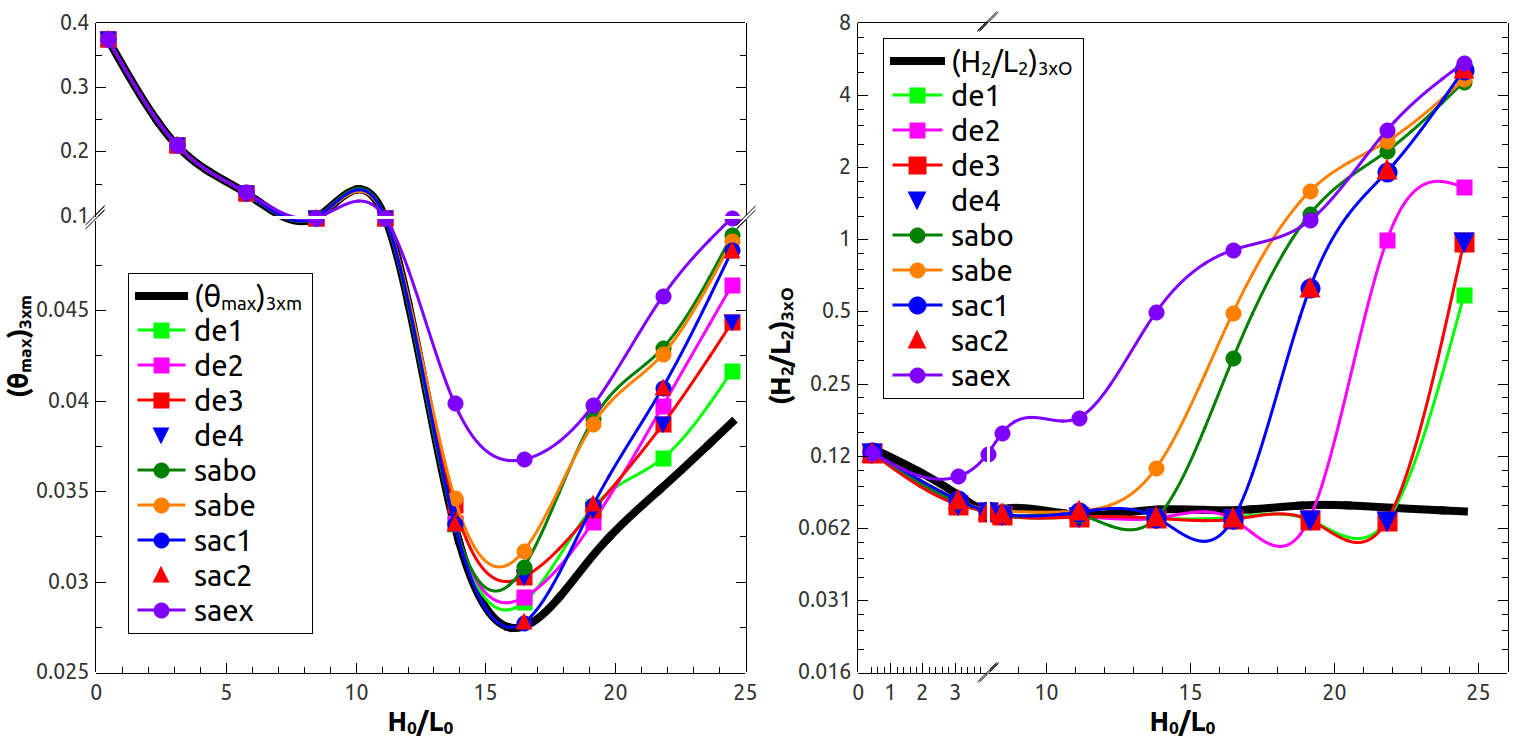
\includegraphics[width=0.9\linewidth]{imgs/4dof/de_sa_h0l0-tmin-4dof.png}
\caption{ {\small Effect of $H_{0}/L_{0}$ over $({\theta}_{max})_{3\times m}$ and $(H_{2}/L_{2})_{3\times o}$ obtained by different versions of DE and SA algorithms. a) Effect over $({\theta}_{max})_{3\times m}$. b) Effect over $(H_{2}/L_{2})_{3\times o}$ }}
\label{figure02}
\end{figure}

Figure \ref{figure02}(b) shows the results of each algorithm analysed in this paper for the effect of  $H_{0}/L_{0}$ over $H_{2}/L_{2}$. In the Fig. \ref{figure02}(b) appears the same tendency observed in the effect of $H_{0}/L_{0}$ over $({\theta}_{max})_{3\times m}$, where the SA algorithm versions achieves the greatest means, mainly after ratio $H_{0}/L_{0}=10$. The DE algorithm has a better performance and the DE1 algorithm version reached a avarage of $(H_{2}/L_{2})_{3\times o}$ more closest to the optimal values of $(H_{2}/L_{2})_{3\times o}$ for each value of  $H_{0}/L_{0}$.

The effect of $H_{0}/L_{0}$ over $(H_{1}/L_{1})_{2\times o}$ and $(S_{1}/H_{0})_{o}$ is showed in the Fig. \ref{figure03}. The curvature represented by the black line in the \ref{figure03} (a) and (b) reproduce the effect of $H_{0}/L_{0}$ over the optimal values of the DOFs investigated. The others curvatures have the averages of this effect produced by each algorithm. In the Fig. \ref{figure03}(a) the results of all algorithm shows a great divergence to the effect of $H_{0}/L_{0}$ on the optimal values of the $(H_{1}/L_{1})_{2\times o}$ for the values of $H_{0}/L_{0}<10$. For high values of $H_{0}/L_{0}$ the averages reached by all algorithm converges to the right effect, except by the SA algorithm version whit the function of cooling schedule Exponential (saex). In the Figure \ref{figure03}(b) the effect of $H_{0}/L_{0}$ over $(S_{1}/H_{0})_{o}$ was better reproduced by the versions of DE algorithm and two versions of SA algorithm (sac1 and sac2). The DE1 and DE2 algorithms achieved the closest effects of the correct curvature, mainly for values of  $H_{0}/L_{0}>15$.

\begin{figure}[H]
\centering
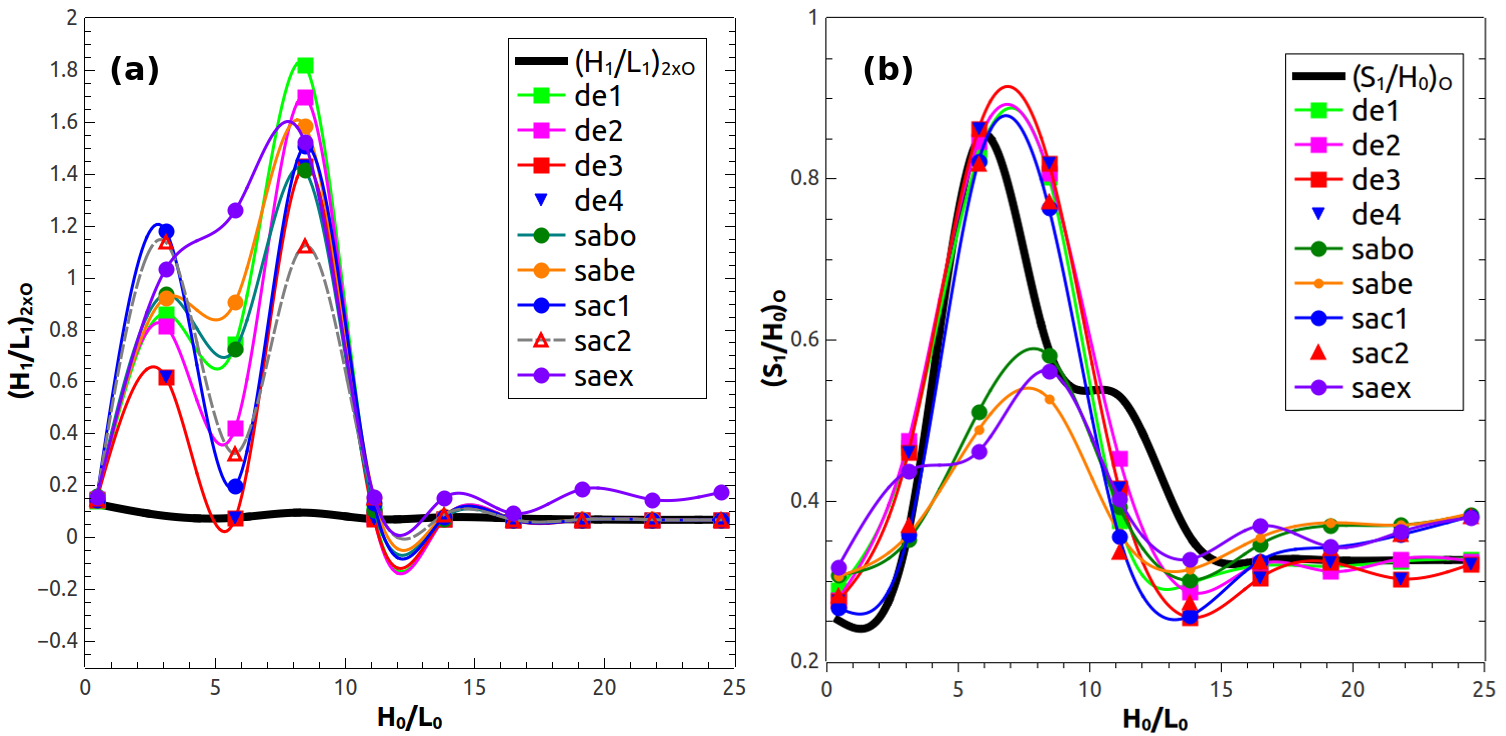
\includegraphics[width=0.9\linewidth]{imgs/4dof/de_sa_h0l0-h1l1-s1h0-4dof.png}
\caption{ {\small Effect of $H_{0}/L_{0}$ over $(H_{1}/L_{1})_{2\times o}$ and $(S_{1}/H_{0})_{o}$ obtained by different versions of DE and SA algorithms. a) Effect over $(H_{1}/L_{1})_{2\times o}$. b) Effect over $(S_{1}/H_{0})_{o}$ }}
\label{figure03}
\end{figure}
For the five DOFs optimization, was run four versions of DE algorithm and the five versions of SA algorithm describes in section 3. All algorithms have the number of iterations, as well as, the evaluation of Objective Function, limited to 300. For each ratio of $H/L$ were performed thirty runs of each algorithm and recorded the maximum excess of temperature four times minimized and the effect of $H/L$ over optimal geometry obtained by the algorithms on each operation. Statistical measures also were stored on the database, as well as, the minimal values of the maximum excess of temperature four times minimized and its respective optimal geometries.

Figure \ref{figure04} shows  the minimal values of the maximum excess of temperature four times minimized represented by the black line, and other curves represents the average of this value reached for each algorithm in the geometric optimization process of five DOFs ($H/L$, $H_{0}/L_{0}$, $H_{1}/L_{1}$, $H_{2}/L_{2}$ and $S_{1}/H_{0}$). Therefore, as can be seen in Fig. \ref{figure04}(a) in comparison whit the results showed in the Fig. \ref{figure04}(b) for SA algorithms versions, the versions of DE algorithm lead to nearest averages to the curve of minimum values of the $({\theta}_{max})_{4\times m}$. For values of $H/L > 0.5$ all algorithm can reproduce the effect of $H/L$ of $({\theta}_{max})_{4\times m}$ with precision. This behavior can be observed in the Fig. \ref{figure05}, where all algorithms achieved the correct effect of $H/L$ over ${(H_{0}/L_{0})_{4\times O}}$.
\begin{figure}[H]
\centering
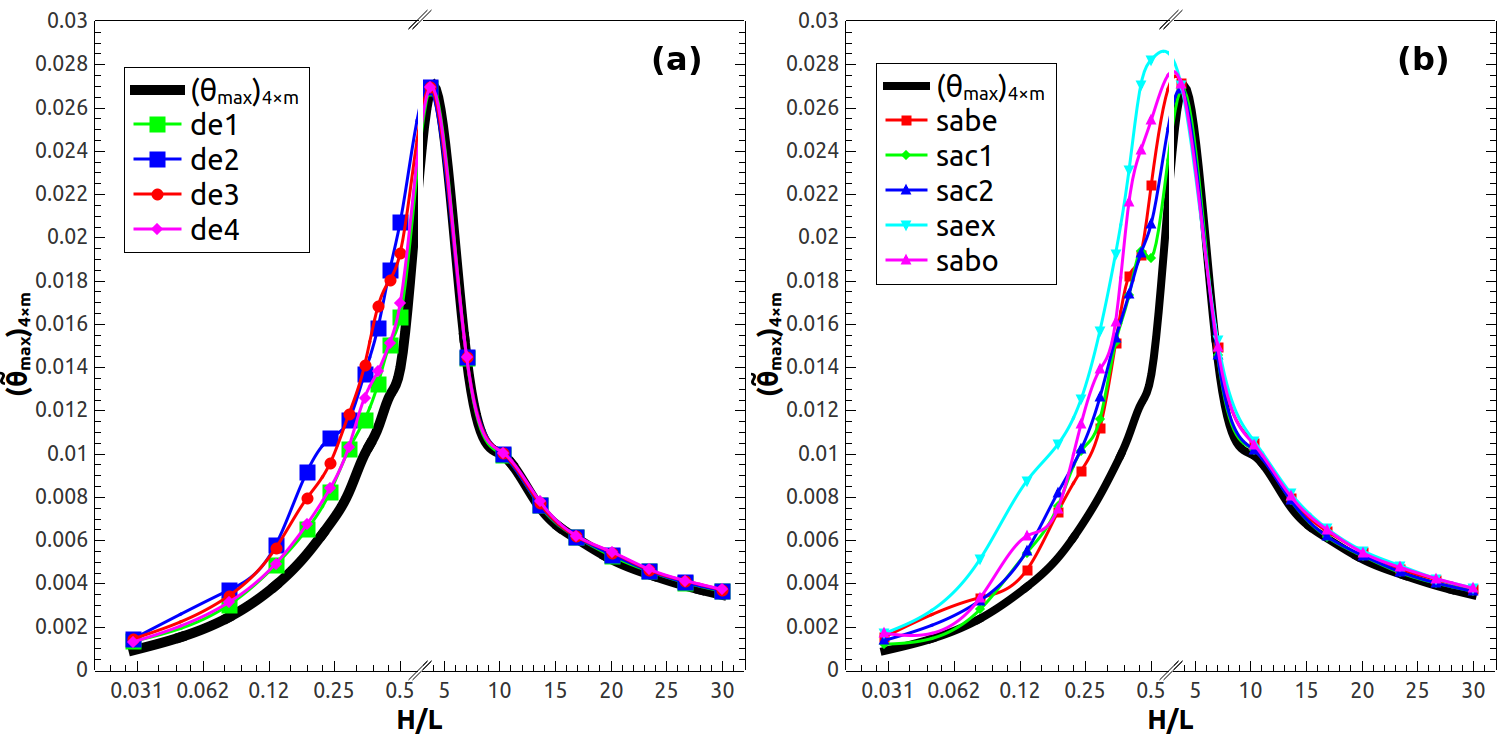
\includegraphics[width=0.9\linewidth]{imgs/5dof/de_sa_hl_tmin.png}
\caption{ {\small Effect of $H/L$ over $({\theta}_{max})_{4\times m}$ obtained by different versions of DE and SA algorithms. a) Versions of DE algorithm. b) Versions of SA algorithm.}}
\label{figure04}
\end{figure}
 

\begin{figure}[H]
\centering
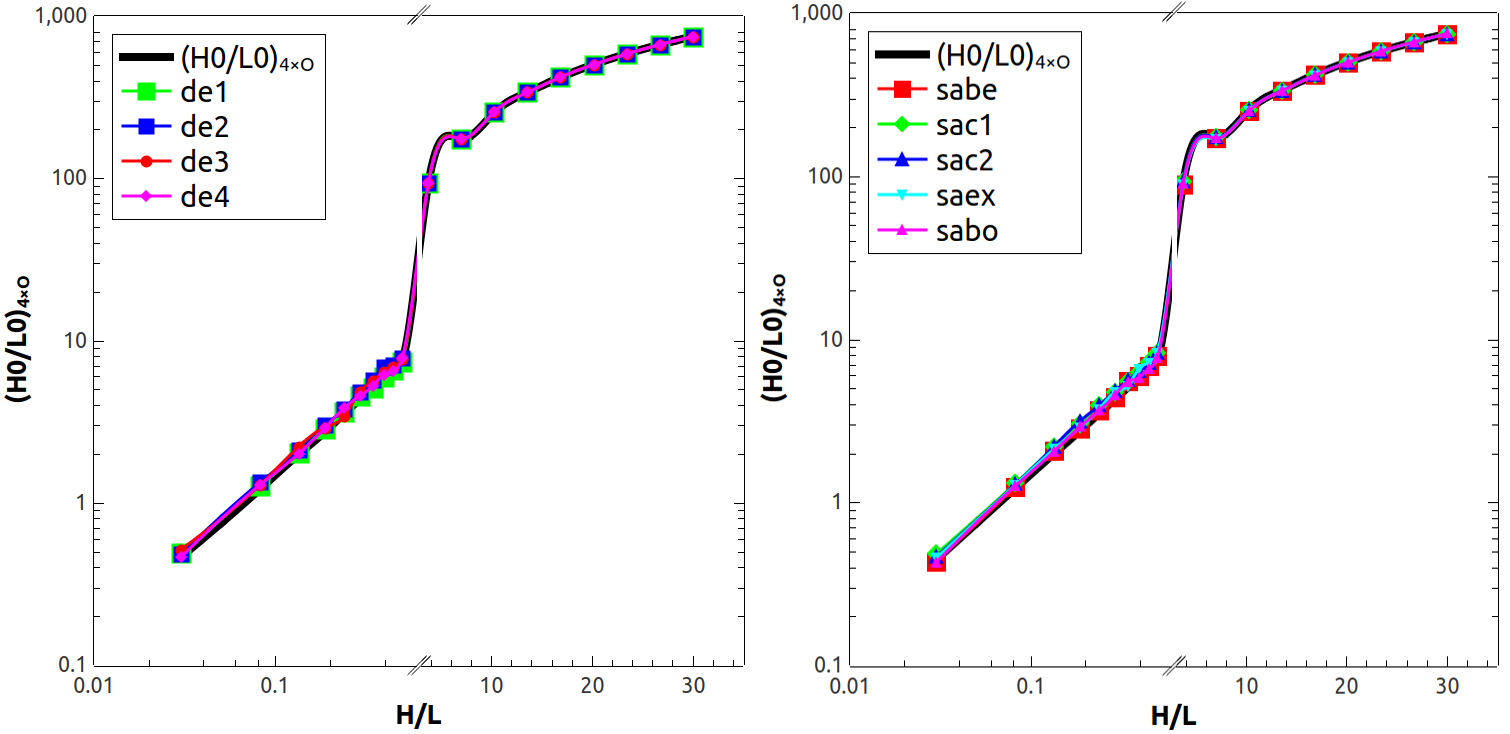
\includegraphics[width=0.9\linewidth]{imgs/5dof/de_sa_hl_h0l0.png}
\caption{ {\small Effect of $H/L$ over ${(H_{0}/L_{0})_{4\times O}}$ obtained by different versions of DE and SA algorithms.  a) Versions of DE algorithm. b) Versions of SA algorithm.}}
\label{figure05}
\end{figure}
Figure \ref{figure06} shows the comparison between the results of the versions of DE algorithm and variants of the SA algorithm for the effect of $H/L$ over ${(H_{2}/L_{2})_{3\times O}}$. In this case, the variations of DE algorithm brings the better results again, except by DE2 version for ratios of $H/L< 0.5$. The results of the SA algorithm versions showed in the Fig. \ref{figure06}(b), diverges of the correct effect of $H/L$ over ${(H_{2}/L_{2})_{3\times O}}$. For the lowest values of ratio $H/L$, neither algorithm reproduce the result correctly, the averages diverge a lot of the effect of $H/L$ over ${(H_{2}/L_{2})_{3\times O}}$. For values of $H/L > 5$ the versions of SA algorithm SAC1 and SAC2 achieved averages more closest to the optimal ratio ${(H_{2}/L_{2})_{3\times O}}$. The difficulty of the versions of SA algorithm to reach the optimal configuration of $H_{2}/L_{2}$ for the lowers ratios of $H/L$ explain the averages of the $({\theta}_{max})_{4\times m}$ showed in the Fig.\ref{figure04}(b).


\begin{figure}[H]
\centering
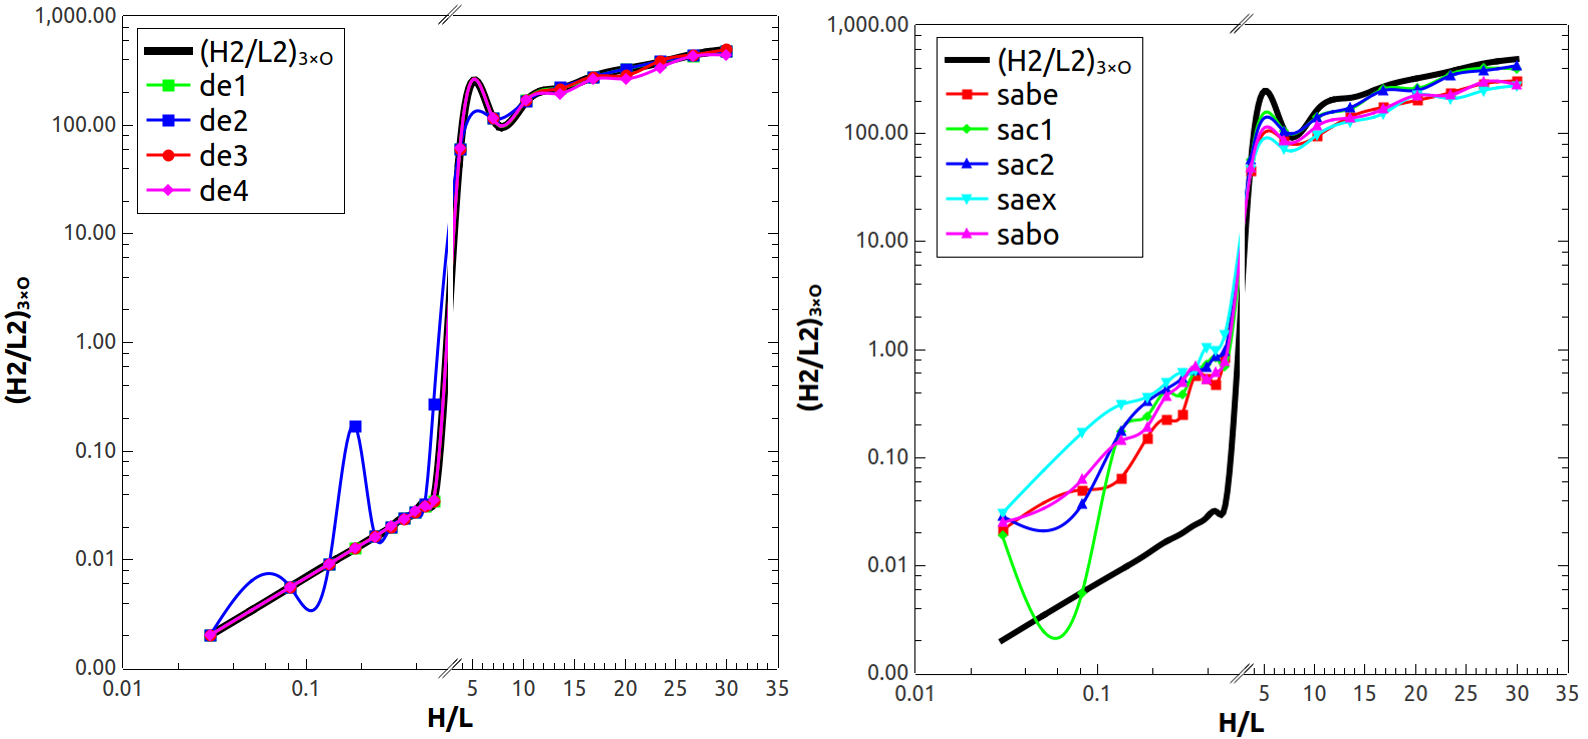
\includegraphics[width=0.9\linewidth]{imgs/5dof/de_sa_hl_h2l2.png}
\caption{ {\small Effect of $H/L$ over ${(H_{2}/L_{2})_{3\times O}}$ obtained by different versions of DE and SA algorithms. a) Versions of DE algorithm. b) Versions of SA algorithm.}}
\label{figure06}
\end{figure}


The effect of $H/L$ over ${(H_{1}/L_{1})_{2\times O}}$ is shown in the Figure \ref{figure07}. The exact effect is represented by the black curve, and the others curvatures represent the averages of the ${(H_{1}/L_{1})_{2\times O}}$ achieved by each algorithm during thirty runs. Fig. \ref{figure07}(a) shows the results of versions of the DE algorithm and in the Fig. \ref{figure07}(b), are shown the results of versions of the SA algorithm. The best results are performed by versions of DE algorithm, that average of ${(H_{1}/L_{1})_{2\times O}}$ fit precisely to the optimal values of ${(H_{1}/L_{1})_{2\times O}}$ for all ratios of $H/L$, except the versions DE3 and DE4 for high values of $H/L$. The versions of the SA algorithm achieve divergent results for this DOF, where the worst performance is given by SAEX, follow by  SABE and SABO. The others versions (SAC1 and SAC2) presents results more nearest of the correct and similar to the results of DE3 and DE4 for high values of $H/L$.


\begin{figure}[H]
\centering
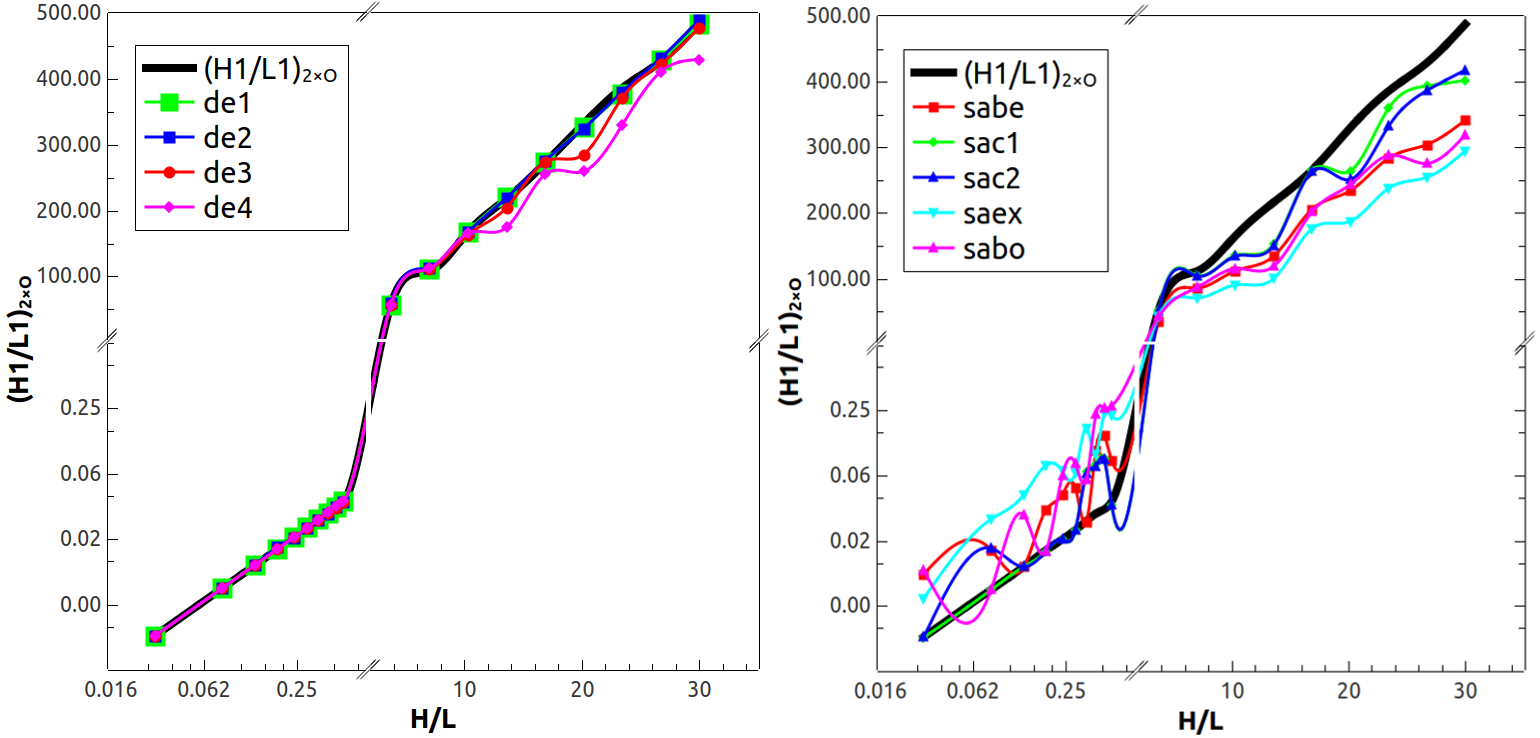
\includegraphics[width=0.9\linewidth]{imgs/5dof/de_sa_hl_h1l1.png}
\caption{ {\small Effect of $H/L$ over ${(H_{1}/L_{1})_{2\times O}}$ obtained by different versions of DE and SA algorithms.  a) Versions of DE algorithm. b) Versions of SA algorithm.}}
\label{figure07}
\end{figure}
In Figure \ref{figure08}, it is possible to note that the results of all algorithms diverge from the optimal values of ${(S_{1}/H_{0})_{2\times O}}$ for all ratios of $H/L$. The results in Fig \ref{figure08}(a) shows that all versions of DE algorithm do not reach the optimal values of ${(S_{1}/H_{0})_{2\times O}}$ for lower ratios of  $H/L$. Moreover, for rates of  $H/L > 0.5$, the versions DE1 and DE2 achieved the best results against DE3 and DE4. The Fig. \ref{figure08}(b) shows that versions of SA algorithm have a great difficulty to achieve the optimal values of ${(S_{1}/H_{0})_{2\times O}}$ for any ratio of  $H/L$ analyzed.
\begin{figure}[H]
\centering
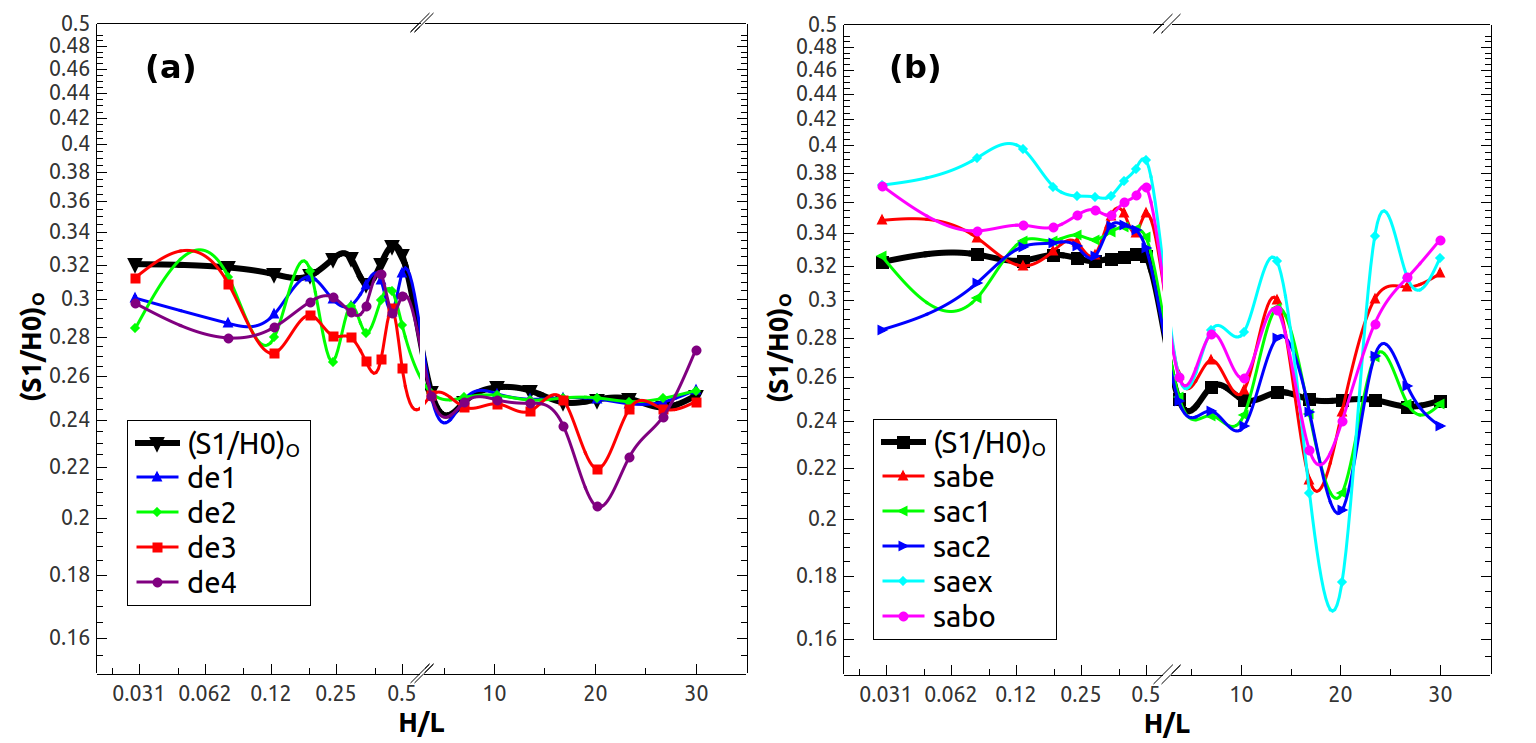
\includegraphics[width=0.9\linewidth]{imgs/5dof/de_sa_hl_s1h0.png}
\caption{ {\small Effect of $H/L$ over ${(S_{1}/H_{0})_{O}}$ obtained by different versions of DE and SA algorithms.  a) Versions of DE algorithm. b) Versions of SA algorithm.}}
\label{figure08}
\end{figure}

\section{CONCLUSIONS}

The present work studied the employment of two meta-heuristic, Simulated Annealing (SA) and Differential Evolution (DE), combined with Constructal Design (CD) to perform a geometric optimization in a heat transfer problem. The problem consists of a Double-T shaped cavity, at minimum temperature prescribe, into a conductive wall with constant heat generation. The geometric optimization problem is conducted by the CD method that defines the Degrees of Freedom (DOFs) and constraints. The purpose is to compare the results of the two heuristics analyzed, as well as, the efficiency to reproduce the right effect of the DOFs over the optimal geometry and thermal resistance of the computational domain.

The SA algorithm versions present results inferior when compared with the performance of the DE version algorithms. However, in an inner comparison between SA versions,  the results show the better performance wich SA algorithms that use the hybrid functions of Cooling Schedule (CS).

The results show that the versions of the DE algorithms represent the results that come closest to the right effect. Moreover, the version DE1 has the most robust results with the lowest average and more approximated of the correct effect of DOFs for the majority cases investigates in this study, as can be seen in the effect of $H_{0}/L_{0}$ over $(H_{2}/L_{2})_{3xo}$ and $({\theta}_{max})_{3\times m}$. For the geometric optimization of five DOF, the versions of DE algorithm also were superior to the results of SA algorithm. The DE1 version have the mean of $({\theta}_{max})_{4\times m}$ more closest to the minimal values, and even in the cases whit more difficult to converge by other algorithms, the results of DE1 were better, as can be observed in the effect of  $H/L$ over ${(S_{1}/H_{0})_{O}}$. Also, it is possible observed, that the DE2 algorithm achieved good results for some cases, as the effect of $H/L$ over ${(S_{1}/H_{0})_{O}}$ and over ${(H_{1}/L_{1})_{2  \times O}}$. However, this version of DE algorithm led to worst results on the effect of $H/L$ over ${(H_{1}/L_{1})_{2  \times O}}$ which influenced the results of $({\theta}_{max})_{4\times m}$. The parameters can explain the difference in the results of this two versions of DE algorithm (DE1 and DE2), whit the same mutation parameter (DE/rand/1/bin), the Crossover rate ($CR$) and amplification factor $F$ (respectively 0.9 and 2 for DE2) are probably the worng parameters to be chosen. An example is that the DE3 also have the worts results compared to the DE4 version of DE algorithm, and it have the same parameters of $CR$ and $F$ that DE2.Therfore, it is possible to conclude that between DE and SA type of algorithm, the DE version have in general a better performance, and among the parameters of DE investigated in present work, the parameters applied in the DE1 version are the best choice, for the problem of cavity analyzed.




\subsection*{\textit{Acknowledgements}}
G. V. Gonzales acknowledges IF-SUL and PPGMC-FURG by support. E. D. dos Santos is sponsored by CNPq. Antônio J. Silva Neto acknowledges the financial support provided by FAPERJ, CNPq and CAPES.


% ------------------------------------------------------------------------

\fontsize{11}{0}\selectfont
\bibliographystyle{xiiiemc}
\bibliography{bibfile}
% ------------------------------------------------------------------------

%For papers written in Portuguese or Spanish.

%\begin{center}
%  TITLE IN ENGLISH
%\end{center}

%\def\abstractname{Abstract}%

%\begin{abstract}
%   Abstract in english
%\end{abstract}

%\keywords{\em{Keywords in english}}

\end{document}
